\documentclass{beamer}

\usepackage{listings}
\lstset{language=C++,basicstyle=\footnotesize\ttfamily,breaklines=true}

% Setup appearance:

% \usetheme{Darmstadt}
% \usefonttheme[onlylarge]{structurebold}
% \setbeamerfont*{frametitle}{size=\normalsize,series=\bfseries}
\setbeamertemplate{navigation symbols}{}

\begin{document}

\begin{frame}{Recap}
  \begin{figure}[htbp]
  \centering
  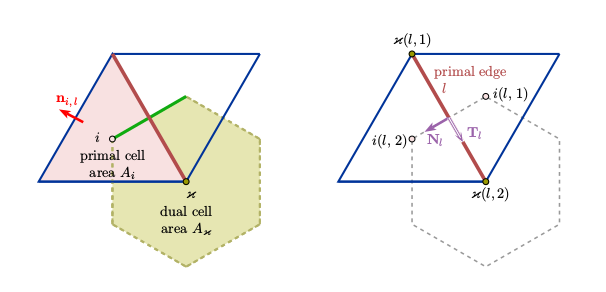
\includegraphics[width=0.8\textwidth]{1.png}
  \end{figure}
  \[\text{div}(v)_i = \frac{1}{A_i}\sum\limits_{l\in \mathcal{E}(i)}v_{n_l}(N_l \cdot n_{i,l})l\]
\end{frame}

\begin{frame}{Recap}
  \begin{figure}[htbp]
  \centering
  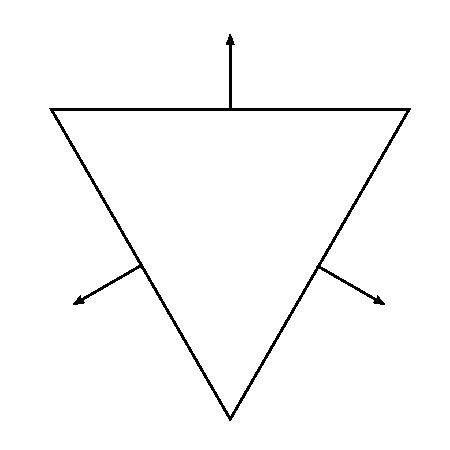
\includegraphics[width=0.3\textwidth]{flow_downward.pdf}
  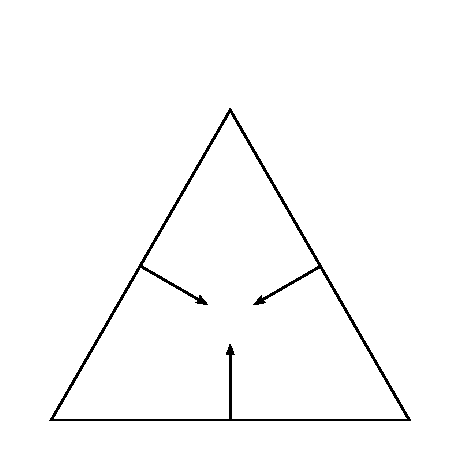
\includegraphics[width=0.3\textwidth]{flow_upward.pdf}
  \end{figure}
  \begin{align*}
    \text{div}(\bm{v})_i& = \frac{1}{A_i}\sum\limits_{l\in\mathcal{E}(i)}v_{n_l}l \quad \text{for downward cells}\\
    \text{div}(\bm{v})_i& = -\frac{1}{A_i}\sum\limits_{l\in\mathcal{E}(i)}v_{n_l}l \quad \text{for upward cells}
  \end{align*}
\end{frame}

\begin{frame}{More operators}
  \begin{equation*}
    \text{div}(v)_i
    &= \frac{1}{A_i}\sum\limits_{l\in \mathcal{E}(i)}v_{n_l}(N_l \cdot n_{i,l})l = \sum\limits_{l\in \mathcal{E}(i)}w_{i,l}v_{n_l}
  \end{equation*}
  edge-to-cell averaging:
  \begin{equation*}
      \bar{\varrho}_i=\sum\limits_{l \in \mathcal{E}(i)}\frac{A_{i,l}}{A_i}\varrho_{l}= \sum\limits_{l\in \mathcal{E}(i)}w_{i,l}v_{n_l}
  \end{equation*}
  cell-to-edge averaging:
  \begin{equation*}
      \breve{\varrho}_l=\sum\limits_{j=1,2}\frac{A_{i(l,j)}}{A_l}\varrho_{i(l,j)}=\sum\limits_{j=1,2}w_{i(l,j)}\varrho_{i(l,j)}
  \end{equation*}
  Used in discretizing the pressure gradient force:
  \begin{equation*}
    \overline{\overline\psi}_l = \frac{A_{i(l,2),l}}{A_l}\psi_{i(l,1)} + \frac{A_{i(l,1),l}}{A_l}\psi_{i(l,2)}=\sum\limits_{j=1,2}w_{i(l,j)}\varrho_{i(l,j)}
  \end{equation*}
\end{frame}

\begin{frame}[fragile]{Fields on multiple locations}
\texttt{\{i,c,j,k\}}

\texttt{\{i,c,j,k,extra\_dimension\}} (new!)

How to access:
\begin{lstlisting}
edges_of_cells_storage_type weights;
weights(i, c, j, k, 2);
\end{lstlisting}

In a functor:
\begin{lstlisting}
typedef in_accessor<1, icosahedral_topology_t::cells, extent<1>, 5 > weights;

using edge_of_cells_dim = dimension< 5 >;
edge_of_cells_dim::Index edge;
eval(weights(edge+2));
\end{lstlisting}
\end{frame}

\begin{frame}[fragile]{Fields on multiple locations}
\begin{lstlisting}{basicstyle=\scriptsize}
template<typename Evaluation>
GT_FUNCTION static void Do(Evaluation const &eval, x_interval)
{
    typedef typename icgrid::get_grid_topology< Evaluation >::type grid_topology_t;

    using edge_of_cells_dim = dimension< 5 >;
    edge_of_cells_dim::Index edge;

    eval(out_cells()) = 0.;
    auto neighbors_offsets = connectivity< cells , edges >::offsets(eval.position()[1]);
    ushort_t e=0;
    for (auto neighbor_offset : neighbors_offsets) {
        eval(out_cells()) += eval(in_edges(neighbor_offset)) * eval(weights(edge+e));
        e++;
    }
}
\end{lstlisting}
\end{frame}

\begin{frame}{Next}
  \begin{itemize}
    \item
  \end{itemize}
\end{frame}
\end{document}
